\documentclass[8pt,a4paper,landscape]{extarticle}
\makeatletter
\def\input@path{{../_shared/}}
\makeatother
\usepackage{cheatsheet}
\usepackage{graphicx}

\begin{document}
\begin{multicols*}{4}

\cheattitle{Algorithms I}{}{BA4}

\begin{thm}[title=Sum of a sequence]
  $\sum_{k=m}^{n} k = \frac{(m+n)(n-m+1)}{2}$\\
  $\sum_{k=m}^{n} z^{k} = \begin{cases} n-m+1 & z=1 \\ \frac{z^m-z^{n+1}}{1-z} & z\ne 1 \end{cases}$\\
  $\displaystyle\sum_{i=1}^{n} \dfrac{1}{i} = \Theta(\log n)$
\end{thm}

\section{Sorting}

\subsection{Insertion Sort}
\begin{lstlisting}
INSERTION-SORT(A, n)
    for j = 2 to n
        key = A[j]
        i = j - 1
        while i > 0 and A[i] > key
            A[i + 1] = A[i]
            i = i - 1
        A[i + 1] = key
\end{lstlisting}

\begin{prop}[title=Runtime \& Loop invariant (like induction)]
In-place. $\Theta(n^2)$ worst, $\Theta(n)$ best. \textbf{Inv:} $A[1..j{-}1]$ sorted.
\textbf{Init:} $j{=}2$, trivial. \textbf{Maint:} key inserted correctly. \textbf{Term:} $A$ sorted.
\end{prop}

\subsection{Merge Sort}
\begin{lstlisting}
MERGE(A, p, q, r)
    n1 = q-p+1; n2 = r-q
    L[1..n1+1] and R[1..n2+1] be new arrays
    for i = 1 to n1: L[i] = A[p+i-1]
    for j = 1 to n2: R[j] = A[q+j]
    L[n1+1] = inf; R[n2+1] = inf
    i = 1; j = 1
    for k = p to r
        if L[i] <= R[j]: A[k] = L[i]; i = i+1
        else: A[k] = R[j]; j = j+1

MERGE-SORT(A, p, r)
    if p < r
        q = floor((p+r)/2)
        MERGE-SORT(A, p, q)
        MERGE-SORT(A, q+1, r)
        MERGE(A, p, q, r)
\end{lstlisting}

\begin{prop}[title=Runtime]
Not in-place. $T(n)=2T(n/2)+\Theta(n)=\Theta(n\lg n)$
\end{prop}

\section{Solving recurrences}

\subsection{The substitution method}
\begin{enumerate}
  \item Guess the form of the solution.
  \item Use \textbf{induction} to find constants \& verify.
\end{enumerate}

\begin{prop}[title=Unintuitive trick]
Sometimes solution is to prove something stronger
\end{prop}

\subsection{Recursion trees}
Draw tree, sum cost per level, sum all levels.

\subsection{Master method}
\begin{thm}[title=Master Theorem]
$T(n)=aT(n/b)+f(n)$, $a\ge1$, $b>1$, $\alpha=\log_b a$:\\[2pt]
\begin{tabular}{@{}l@{$\;\Rightarrow\;$}l@{}}
$f=O(n^{\alpha-\varepsilon})$                        & $T=\Theta(n^\alpha)$ \\
$f=\Theta(n^{\alpha})$                               & $T=\Theta(n^\alpha\log n)$ \\
$f=\Omega(n^{\alpha+\varepsilon})$, $af(n/b)\le cf(n)$ & $T=\Theta(f(n))$ \\
\end{tabular}
\end{thm}

\section{Maximum-Subarray Problem}

{\centering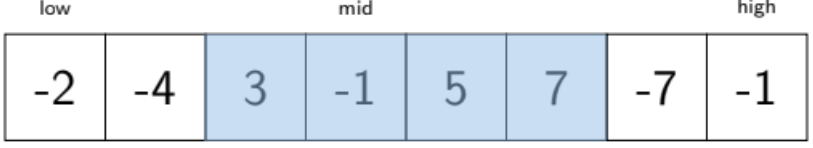
\includegraphics[width=\linewidth,height=1.5cm,keepaspectratio]{images/max-crossing-subarray.png}\par}

\begin{lstlisting}
FIND-MAX-CROSSING-SUBARRAY(A, low, mid, high)
    ls=-inf; rs=-inf; sum=0
    for i=mid downto low      // max: form A[i..mid]
        sum+=A[i]
        if sum>ls: ls=sum; ml=i
    sum=0
    for j=mid+1 to high     // max: form A[mid+1..j]
        sum+=A[j]
        if sum>rs: rs=sum; mr=j
    return (ml, mr, ls+rs)

FIND-MAXIMUM-SUBARRAY(A, low, high)
    if high==low: return (low, high, A[low])
    mid=floor((low+high)/2)
    (ll,lh,ls) = FIND-MAXIMUM-SUBARRAY(A,low,mid)
    (rl,rh,rs) = FIND-MAXIMUM-SUBARRAY(A,mid+1,high)
    (cl,ch,cs) = FIND-MAX-CROSSING-SUBARRAY(A,low,mid,high)
    if ls>=rs and ls>=cs: return (ll,lh,ls)
    elseif rs>=cs: return (rl,rh,rs)
    else: return (cl,ch,cs)
\end{lstlisting}

\begin{prop}[title=Runtime]
$T(n)=2T(n/2)+\Theta(n)=\Theta(n\lg n)$
\end{prop}

\section{Matrix Multiplication}

$c_{ij}=\sum_{k=1}^n a_{ik}b_{kj}$. \textbf{Naive:} $\Theta(n^3)$ time, $\Theta(n^2)$ space.

\subsection{Raw Divide-and-Conquer}
\begin{prop}[title=Runtime]
8 calls: $T(n)=8T(n/2)+\Theta(n^2)=\Theta(n^3)$
\end{prop}

\subsection{Strassen's Algorithm using Divide-and-Conquer}
Only \textbf{7} recursive calls. Partition as before, compute:
\begin{lstlisting}
M1=(A11+A22)(B11+B22)  M5=(A11+A12)B22
M2=(A21+A22)B11        M6=(A21-A11)(B11+B12)
M3=A11(B12-B22)        M7=(A12-A22)(B21+B22)
M4=A22(B21-B11)
C11=M1+M4-M5+M7  C12=M3+M5
C21=M2+M4        C22=M1-M2+M3+M6
\end{lstlisting}
\begin{prop}[title=Runtime]
$T(n)=7T(n/2)+\Theta(n^2)=\Theta(n^{\lg 7})\approx\Theta(n^{2.807})$
\end{prop}

\section{Karatsuba's Algorithm}
\textbf{Problem:} multiply two $n$-digit integers $x,y$ in base $b$.

\textbf{Divide:} split each number in two halves of $n/2$ digits:
\[x=x_H b^{n/2}+x_L \qquad y=y_H b^{n/2}+y_L\]
\[x\cdot y=x_Hy_H\cdot b^n+(x_Hy_L+x_Ly_H)\cdot b^{n/2}+x_Ly_L\]

\textbf{Key:} naively 4 products, but:
\[x_Hy_L+x_Ly_H=(x_H{+}x_L)(y_H{+}y_L)-x_Hy_H-x_Ly_L\]
So only \textbf{3 recursive multiplications} needed.

\begin{prop}[title=Runtime]
$T(n)=3T(n/2)+\Theta(n)=\Theta(n^{\log_2 3})\approx\Theta(n^{1.585})$
\end{prop}

\section{Heaps}
\subsection{Max-Heapify}
Assumes subtrees rooted at \texttt{LEFT}$(i)$ and \texttt{RIGHT}$(i)$ are already max-heaps.

\begin{lstlisting}
MAX-HEAPIFY(A, i, n)
    l = LEFT(i)
    r = RIGHT(i)
    if l <= n and A[l] > A[i]
        largest = l
    else largest = i
    if r <= n and A[r] > A[largest]
        largest = r
    if largest != i
        exchange A[i] with A[largest]
        MAX-HEAPIFY(A, largest, n)
\end{lstlisting}

\begin{prop}[title=Runtime]
$T(n) \le T(2n/3) + \Theta(1) = O(\lg n)$
\end{prop}

\subsection{Build-Max-Heap}

\begin{lstlisting}
BUILD-MAX-HEAP(A, n)
    for i = floor(n/2) downto 1
        MAX-HEAPIFY(A, i, n)
\end{lstlisting}

\begin{prop}[title=Runtime]
$O(n)$ (tighter than the naive $O(n \lg n)$)
\end{prop}

\subsection{Heapsort}

\begin{lstlisting}
HEAPSORT(A, n)
    BUILD-MAX-HEAP(A, n)
    for i = n downto 2
        exchange A[1] with A[i]
        MAX-HEAPIFY(A, 1, i-1)
\end{lstlisting}

\begin{prop}[title=Runtime]
$O(n \lg n)$, in-place.
\end{prop}

\subsection{Implementation of priority queue}

\begin{lstlisting}
HEAP-EXTRACT-MAX(A, n) # error if n < 1
    max, A[1] = A[1], A[n]
    MAX-HEAPIFY(A, 1, n-1)
    return max

HEAP-INCREASE-KEY(A, i, key) # error if key < A[i]
    A[i] = key
    while i > 1 and A[PARENT(i)] < A[i]
        exchange A[i] with A[PARENT(i)]
        i = PARENT(i)

MAX-HEAP-INSERT(A, key, n)
    n = n + 1
    A[n] = -inf
    HEAP-INCREASE-KEY(A, n, key)
\end{lstlisting}

\begin{prop}[title=Runtimes]
\texttt{Insert}: $O(\lg n)$, \texttt{Maximum}: $O(1)$, \texttt{Extract-Max}: $O(\lg n)$, \texttt{Increase-Key}: $O(\lg n)$
\end{prop}

\section{Data Structures for items}

\textbf{Stack} (LIFO): +: \texttt{PUSH(S,x)}, -: \texttt{POP(S)}.
\textbf{Queue} (FIFO): +: \texttt{ENQUEUE(Q,x)}, -: \texttt{DEQUEUE(Q)}.

\newpage

\section{Data Structures for Disjoint Sets}
Each set identified by a representative.

\begin{defn}[title=Operations]
\begin{itemize}
  \item \texttt{MAKE-SET(x)}: $S_i = \{x\}$, add to $\mathcal{S}$
\end{itemize}
Let $x \in S_x$, $y \in S_y$
\begin{itemize}
  \item \texttt{UNION(x, y)}: $\mathcal{S} = \mathcal{S} \setminus \{S_x, S_y\} \cup \{S_x \cup S_y\}$
  \item \texttt{FIND(x)}: return representative of $x$ in $S_x$
\end{itemize}
\end{defn}

\begin{lstlisting}
CONNECTED-COMPONENTS(G)
    for each vertex v in G.V
        MAKE-SET(v)
    for each edge (u, v) in G.E
        if FIND(u) != FIND(v)
            UNION(u, v)
\end{lstlisting}

\section{Traversing/Searching a Graph G=(V,E)}

\subsection{BFS - Breadth-First Search}

\begin{lstlisting}
BFS(G, s)
    for each u in G.V - {s}
        u.color = WHITE; u.d = inf; u.pi = NIL
    s.color = GRAY; s.d = 0; s.pi = NIL
    Q = {s}
    while Q != {}
        u = DEQUEUE(Q)
        for each v in G.Adj[u]
            if v.color == WHITE
                v.color = GRAY
                v.d = u.d + 1; v.pi = u
                ENQUEUE(Q, v)
        u.color = BLACK
\end{lstlisting}

\begin{prop}[title=BFS properties]
Search for all vertices from $s$. Runtime: $O(V+E)$.
\end{prop}

\subsection{DFS - Depth-First Search}

\begin{lstlisting}
DFS(G)
    for each u in G.V: u.color = WHITE
    time = 0
    for each u in G.V
        if u.color == WHITE: DFS-VISIT(G, u)

DFS-VISIT(G, u)
    time = time + 1; u.d = time
    u.color = GRAY
    for each v in G.Adj[u]
        if v.color == WHITE: DFS-VISIT(v)
    u.color = BLACK
    time = time + 1; u.f = time
\end{lstlisting}

\begin{prop}[title=Runtime]
$\Theta(V+E)$
\end{prop}

\begin{thm}[title=Parenthesis theorem]
For all $u,v$, exactly one of:
\begin{itemize}
  \item \textbf{Neither ances.:} $u.d<u.f<v.d<v.f$ (or >)
  \item \textbf{$v$ descendant of $u$:} $u.d<v.d<v.f<u.f$
  \item \textbf{$u$ descendant of $v$:} $v.d<u.d<u.f<v.f$
\end{itemize}
\end{thm}

\begin{defn}[title=Classification of edges]
\textcolor{orange}{\textbf{Tree:}} found by exploring $(u,v)$ in DF forest\\
\textcolor{blue}{\textbf{Back:}} $(u,v)$, $u$ descendant of $v$\\
\textcolor{red}{\textbf{Forward:}} $(u,v)$, $v$ desc.\ of $u$, not tree edge\\
\textcolor{green!60!black}{\textbf{Cross:}} any other edge\\
\textbf{UDG:} only tree/back edges. | \textbf{DAG:} no back edge.
\end{defn}
\begin{center} % A retirer si besoin d'espace
  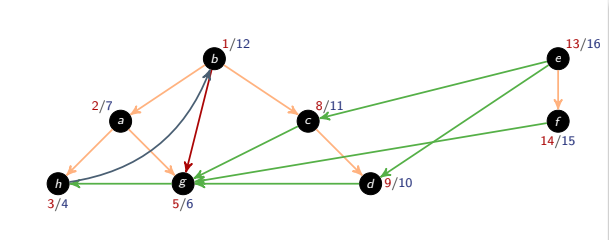
\includegraphics[width=\linewidth]{images/classification_of_edges.png}
\end{center}

\subsection{Topological sort}

\begin{lstlisting}
TOPOLOGICAL-SORT(G):
    Call DFS(G) to compute v.f for all v in G.V
    Output vertices in order of decreasing v.f
\end{lstlisting}

\begin{prop}[title=Runtime]
Same as DFS: $\Theta(V+E)$
\end{prop}

\subsection{Strongly connected components (SCC)}
\begin{lstlisting}
SCC(G):
    Call DFS(G) to compute u.f for all u
    Compute G^T (with all edges reversed)
    Call DFS(G^T), visiting vertices in
      decreasing u.f order
    Output each tree in DFS forest = one SCC
\end{lstlisting}

\begin{prop}[title=Runtime]
Same as DFS: $\Theta(V+E)$
\end{prop}

\section{Flow network}

\begin{thm}[title=Capacity constraint]
$\forall u,v\in V$, $0\le f(u,v)\le c(u,v)$
\end{thm}

\begin{defn}[title=Cut]
Partition of $V$ into two disjoint sets $S$ and $T$ such that $s\in S$ and $t\in T$. $c(S,T)=\sum_{u\in S, v\in T} c(u,v)$.
\end{defn}

\subsection{Maximum flow problem - Ford-Fulkerson method}

\begin{prop}[title={Residual network $G_f=(V,E_f)$}]
$c_f(u,v)$: additional flow possible (forward edge) or removable (backward edge).
\end{prop}

\begin{lstlisting}
FORD-FULKERSON-METHOD(G, s, t)
    initialize flow f to 0
    while exists an augmenting path p in G_f
        b = bottleneck(p)
        augment flow along p by b
    return f
\end{lstlisting}

\subsection{Min cut problem}

\begin{thm}[title=Max-flow min-cut theorem ($\Leftrightarrow$)]
\begin{itemize}
  \item f is the maximum flow
  \item $G_f$ has no augmenting path
  \item $|f| = c(S,T)$ for a minimum cut (S, T)
\end{itemize}
\end{thm}

\subsection{Applications of max flow}
\begin{prop}[title=Bipartite matching as flow]
$G=(V,E)$, $V=L\cup R$. Connect $s\to\forall u\in L$ and $\forall v\in R\to t$, all capacities 1. Run Ford-Fulkerson.
\end{prop}

\begin{prop}[title=Edge-disjoint paths]
Max \# edge-disjoint paths from $s$ to $t$ = min edges to remove to disconnect $s$ from $t$ = max flow (c=1).
\end{prop}


% ============================================================
\section{Spanning Trees}

\begin{defn}[title=Definition]
Set $T$ of edges that is acyclic and spanning (connects all vertices of $G$).
\textbf{Goal of MST problem: }Find a spanning tree of min total weight.
\end{defn}

\begin{thm}[title=Cut property (safe edge)]
Given any cut, a minimum-weight crossing edge belongs to some MST.
\end{thm}

\subsection{Prim's algorithm}
\begin{lstlisting}
PRIM(G, w, r)    // G undirected ; w: E -> R weights
    Q = {}          // min-priority queue (min-heap)
    for each u in G.V:
        u.key = inf
        u.pi = NIL             // u.pi = parent in T
        INSERT(Q, u)
    DECREASE-KEY(Q, r, 0)               // r.key = 0
    while Q != {}:
        u = EXTRACT-MIN(Q)
        for each v in G.Adj[u]:
            if v in Q and w(u,v) < v.key:
                v.pi = u
                DECREASE-KEY(Q, v, w(u,v))
\end{lstlisting}

\begin{thm}[title=Why does it work?]
T is always a subtree of a MST.
\end{thm}

\begin{prop}[title=Prim's runtime]
$O(E\lg V)$ with binary heap. $O(V\lg V+E)$ with Fibonacci heap.
\end{prop}

\subsection{Kruskal's algorithm}
\begin{lstlisting}
KRUSKAL(G, w)
    A = {}
    for v in G.V: MAKE-SET(v)
    sort G.E by w non-decreasing
    for (u, v) in G.E (sorted):
        if FIND(u) != FIND(v)
            A += {(u,v)}; UNION(u, v)
    return A
\end{lstlisting}

\begin{thm}[title=Why does it work?]
T is always a sub-forest of a MST.
\end{thm}

\begin{prop}[title=Kruskal's runtime]
$O(E\lg E) = O(E\lg V)$ (sorting dominates).
\end{prop}

% ============================================================

\section{Shortest Paths}

\begin{defn}[title=Problem variants]
\begin{itemize}
  \item \kv{Single-source}{from $s$ to all vertices}
  \item \kv{Single-dest.}{reverse edges $\to$ single-source}
  \item \kv{Single-pair}{no better worst case than single-s.}
  \item \kv{All-pairs}{solve single-source for each vertex}
\end{itemize}
\end{defn}

\begin{warn}[title=Negative weights]
Allowed but no negative-weight cycle.
\end{warn}

\begin{prop}[title=Optimal substructure]
Any subpath of a shortest path is itself a shortest path (proof by contradiction).
\end{prop}

\begin{warn}[title=Helpful tools]
\begin{itemize}
  \item $d(v) > $ path cost from s to v (upper bound)
  \item $\pi(v) $ is the predecessor of v in this shortest path
\end{itemize}
\end{warn}

\begin{lstlisting}
INIT-SINGLE-SOURCE(G, s)
    s.d = 0
    for v in G.V: v.d = inf; v.pi = NIL

RELAX(u, v, w)
    if v.d > u.d + w(u, v)
        v.d = u.d + w(u, v); v.pi = u
\end{lstlisting}

\subsection{Bellman-Ford}

\begin{lstlisting}
BELLMAN-FORD(G, w, s)
    INIT-SINGLE-SOURCE(G, s)
    for i = 1 to |G.V| - 1
        for (u, v) in G.E: 
            RELAX(u, v, w)
\end{lstlisting}

\begin{thm}[title=Correctness]
\textbf{Invariant:} $l$(v) is at most the length of the shortest path from s to v using at most i edges after the i’th iteration. 
\textbf{Intuition:} Après l'itération i, pour tout sommet v dont le plus court chemin depuis s utilise au plus i arêtes, $l$(v) vaut déjà sa valeur finale.
\end{thm}

\begin{prop}[title=Negative cycle detection]
Run a $|V|$-th iteration: if any edge $(u,v)$ can still be relaxed, the shortest path to $v$ would require more than $|V|-1$ edges, implying a cycle. Since relaxing it decreases the cost, that cycle must be negative.
\end{prop}

\begin{prop}[title=Runtime]
$\Theta(E\cdot V)$. Good for distributed routing: each vertex repeatedly asks neighbors for best path.
\end{prop}

\subsection{Dijkstra's Algorithm}
Non-negative weights only. (an algo like Prim's)

\begin{lstlisting}
DIJKSTRA(G, w, s)
    INIT-SINGLE-SOURCE(G, s)
    S = {}
    Q = G.V   // min-priority queue (sorted by d(v))
    while Q != {}:
        u = EXTRACT-MIN(Q)
        S = S U {u}
        for each vertex v in G.Adj[u]:
            RELAX(u, v, w)
\end{lstlisting}

\begin{thm}[title=Loop invariant (correctness)]
At the start of each iteration, we have for all $v \in S$ that the distance $v.d$ from $s$ to $v$ is equal to the shortest path from $s$ to $v$.
\end{thm}

\begin{prop}[title=Runtime]
The runtime is the same as Prim's algorithm.
\end{prop}

% ============================================================
\section{Probabilistic Analysis}

Worst case rarely happens. Randomization helps avoid worst-case and adversarial inputs (e.g., random pivot in quicksort). Also necessary in cryptography.

\begin{defn}[title=Indicator RV]
\[I\{A\} = \begin{cases}1 & A\text{ occurs}\\0 & \text{otherwise}\end{cases}\]
\textbf{Lemma:} $\E[I\{A\}] = P\{A\}$
\end{defn}

\begin{prop}[title=Hiring Problem]
Expected $\#$ of hires is $O(\ln n)$ vs worst case $O(n)$.
\end{prop}

\begin{prop}[title=Birthday lemma]
Prob.\ of \emph{no} collision among $q$ items drawn uniformly from $[n]$:
$\leq e^{-q(q-1)/(2n)}$.
\end{prop}

% ============================================================
\section{Data Structure: Hash Tables}
Insert, Delete and Search in $O(1)$

\begin{defn}[title=Hash function]
$h: U\to\{0,\ldots,m{-}1\}$ maps key universe to $m$ slots.\\
\textbf{Collision:} $h(k_1)=h(k_2)$ with $k_1\neq k_2$.\\
\textbf{Load factor:} $\alpha = n/m$ (number of keys / slots).
\end{defn}

\begin{prop}[title=Chaining (collision resolution)]
Each slot: linked list of keys.
\end{prop}

% ============================================================
\section{Quick Sort}
\begin{thm}[title=Loop invariant of Partitioning]
\begin{enumerate}
  \item All entries in A[p...i] are <= pivot
  \item All entries in A[i+1...j] are > pivot
  \item A[r] = pivot
\end{enumerate}
\end{thm}

\begin{lstlisting}
PARTITION(A,p,r)
    x = A[r]
    i = p-1
    for j = p to r - 1
        if A[j] <= x
            i = i + 1
            exchange A[i] with A[j]
    exchange A[i+1] with A[r]
    return i+1

QUICKSORT(A, p, r)
    if p < r
        q = PARTITION(A, p, r)
        QUICKSORT(A, p, q-1)
        QUICKSORT(A, q+1, r)
\end{lstlisting}

\begin{prop}[title=Runtime]
In-place $\Theta(n^2)$ worst, $\Theta(n\lg(n))$ on best/average
\end{prop}


\subsection{Randomized version}
\begin{lstlisting}
RANDOMIZED-PARTITION(A, p, r)
    i = RANDOM(p, r)
    exchange A[r] with A[i]
    return PARTITION(A, p, r)

RANDOMIZED-QUICKSORT(A, p, r)
    if p < r
        q = RANDOMIZED-PARTITION(A, p, r)
        RANDOMIZED-QUICKSORT(A, p, q-1)
        RANDOMIZED-QUICKSORT(A, q+1, r)
\end{lstlisting}
It changes how likely the worst case is to occur.

% ============================================================
\section{Logarithm Identities}
% ============================================================

\begin{prop}[title=Key Identities]
\kv{Change of base}{$\log_b(n) = \dfrac{\log_2(n)}{\log_2(b)}$}
\kv{Product}{$\log(a \times b) = \log(a) + \log(b)$}
\end{prop}


\end{multicols*}
\end{document}
